\documentclass[conference]{IEEEtran}
\IEEEoverridecommandlockouts
% The preceding line is only needed to identify funding in the first footnote. If that is unneeded, please comment it out.
\usepackage{array}
\newcolumntype{C}[1]{>{\centering\arraybackslash}p{#1}}
\newcolumntype{M}[1]{>{\centering\arraybackslash}m{#1}}
\usepackage{cite}
\usepackage{amsmath}
\usepackage{caption}
\usepackage{subcaption}
\usepackage[autostyle]{csquotes}
\usepackage{upquote}
\usepackage{hyperref}
\usepackage{color}
\usepackage{soul}
\usepackage{multirow}

\usepackage{amsmath,amssymb,amsfonts}
\usepackage{algorithmic}
\usepackage{graphicx}
\usepackage{textcomp}
\def\BibTeX{{\rm B\kern-.05em{\sc i\kern-.025em b}\kern-.08em
    T\kern-.1667em\lower.7ex\hbox{E}\kern-.125emX}}
\begin{document}

\title{Deep Finger Texture Learning for Verifying People\\
%{\footnotesize \textsuperscript{*}Note: Sub-titles are not captured in Xplore and
%should not be used}
%\thanks{Identify applicable funding agency here. If none, delete this.}
}

\author{\IEEEauthorblockN{Raid R. Omar}
\IEEEauthorblockA{\textit{Department of Computer Science} \\
\IEEEauthorblockA{\textit{and Information Systems,} \\
\textit{Birkbeck, University of London}\\
London, UK \\
raid@dcs.bbk.ac.uk}}
\and
\IEEEauthorblockN{Tingting Han}
\IEEEauthorblockA{\textit{Department of Computer Science} \\
\IEEEauthorblockA{\textit{and Information Systems,} \\
\textit{Birkbeck, University of London}\\
London, UK \\
tingting@dcs.bbk.ac.uk}}
\and
\IEEEauthorblockN{Taolue Chen}
\IEEEauthorblockA{\textit{Department of Computer Science} \\
\IEEEauthorblockA{\textit{and Information Systems,} \\
\textit{Birkbeck, University of London}\\
London, UK \\
taolue@dcs.bbk.ac.uk}}
}

\maketitle

\begin{abstract}
Finger Texture (FT) is currently attracting significant attentions in the case of human recognition. Finger texture covers the area between the lower knuckle of the finger and the upper phalanx before the fingerprint. It involves rich features  which can be efficiently used as a biometric characteristic. In this paper, we will contribute to this growing area by proposing a new verification approach named Deep Finger Texture Learning (DFTL). To the best of our knowledge, this is the first time that the deep learning is employed for recognizing people by using the FT characteristic. Four databases have been used to evaluate the proposed method: the Hong Kong Polytechnic University Contact-free 3D/2D (PolyU2D), Indian Institute of Technology Delhi (IITD), CASIA Blue spectral (CASIA-BLU) corresponding to spectral 460nm and CASIA White spectral (CASIA-WHT) from the CASIA Multi-Spectral images database. The obtaining results have shown superior performance compared with recent publications. The Successful Verification Accuracies (SVAs) have attained 100\%, 98.65\%, 100\% and 98\% for the four databases of PolyU2D, IITD, CASIA-BLU and CASIA-WHT, respectively. 
\end{abstract}

\begin{IEEEkeywords}
Finger Texture; Deep learning; Verification
\end{IEEEkeywords}

\section{Introduction}
In recent years, different finger patterns have been investigated in the case of personal recognition. Examples of these are finger geometry \cite{Liu2015Hand}, finger vein \cite{Lu2014Finger}, finger outer knuckle \cite{Kumar2014Importance} and Finger Texture (FT) \cite{Al-Nima2017finger} \cite{Al-Nima2017Robust}. Using the FTs of four or five fingers in terms of individual verification has been confirmed to be valuable \cite{Al-Nima2017efficient} \cite{Al-Nima2016ANovel} \cite{Al-Nima2015Human}. 

Fundamentally, the FT is located between the upper phalanx (directly under the fingerprint) and the lower knuckle (the base of the finger). It composes of three phalanxes and three knuckles on the inner surface of a little, ring, middle or index finger and it consists of two phalanxes and two knuckles on the inner surface of a thumb. Thus, it involves different qualified patterns. The main FT positions in a hand image are given in Fig. \ref{fig:FT_locations}. \marginpar{insert a picture to show phalanx, knuckle, etc}

Moreover, the FT patterns are unique and reliable between people and even between identical twins. It generally includes visible principal lines and wrinkles \cite{Bhaskar2014Hand}. A low resolution or an inexpensive acquisition device can be used to collect the FT images \cite{Michael2010Robust}. All FT patterns have natural protection as they are positioned inside the fist \cite{Al-Nima2015Human}. 
\begin{figure}[!h]
    \centering
    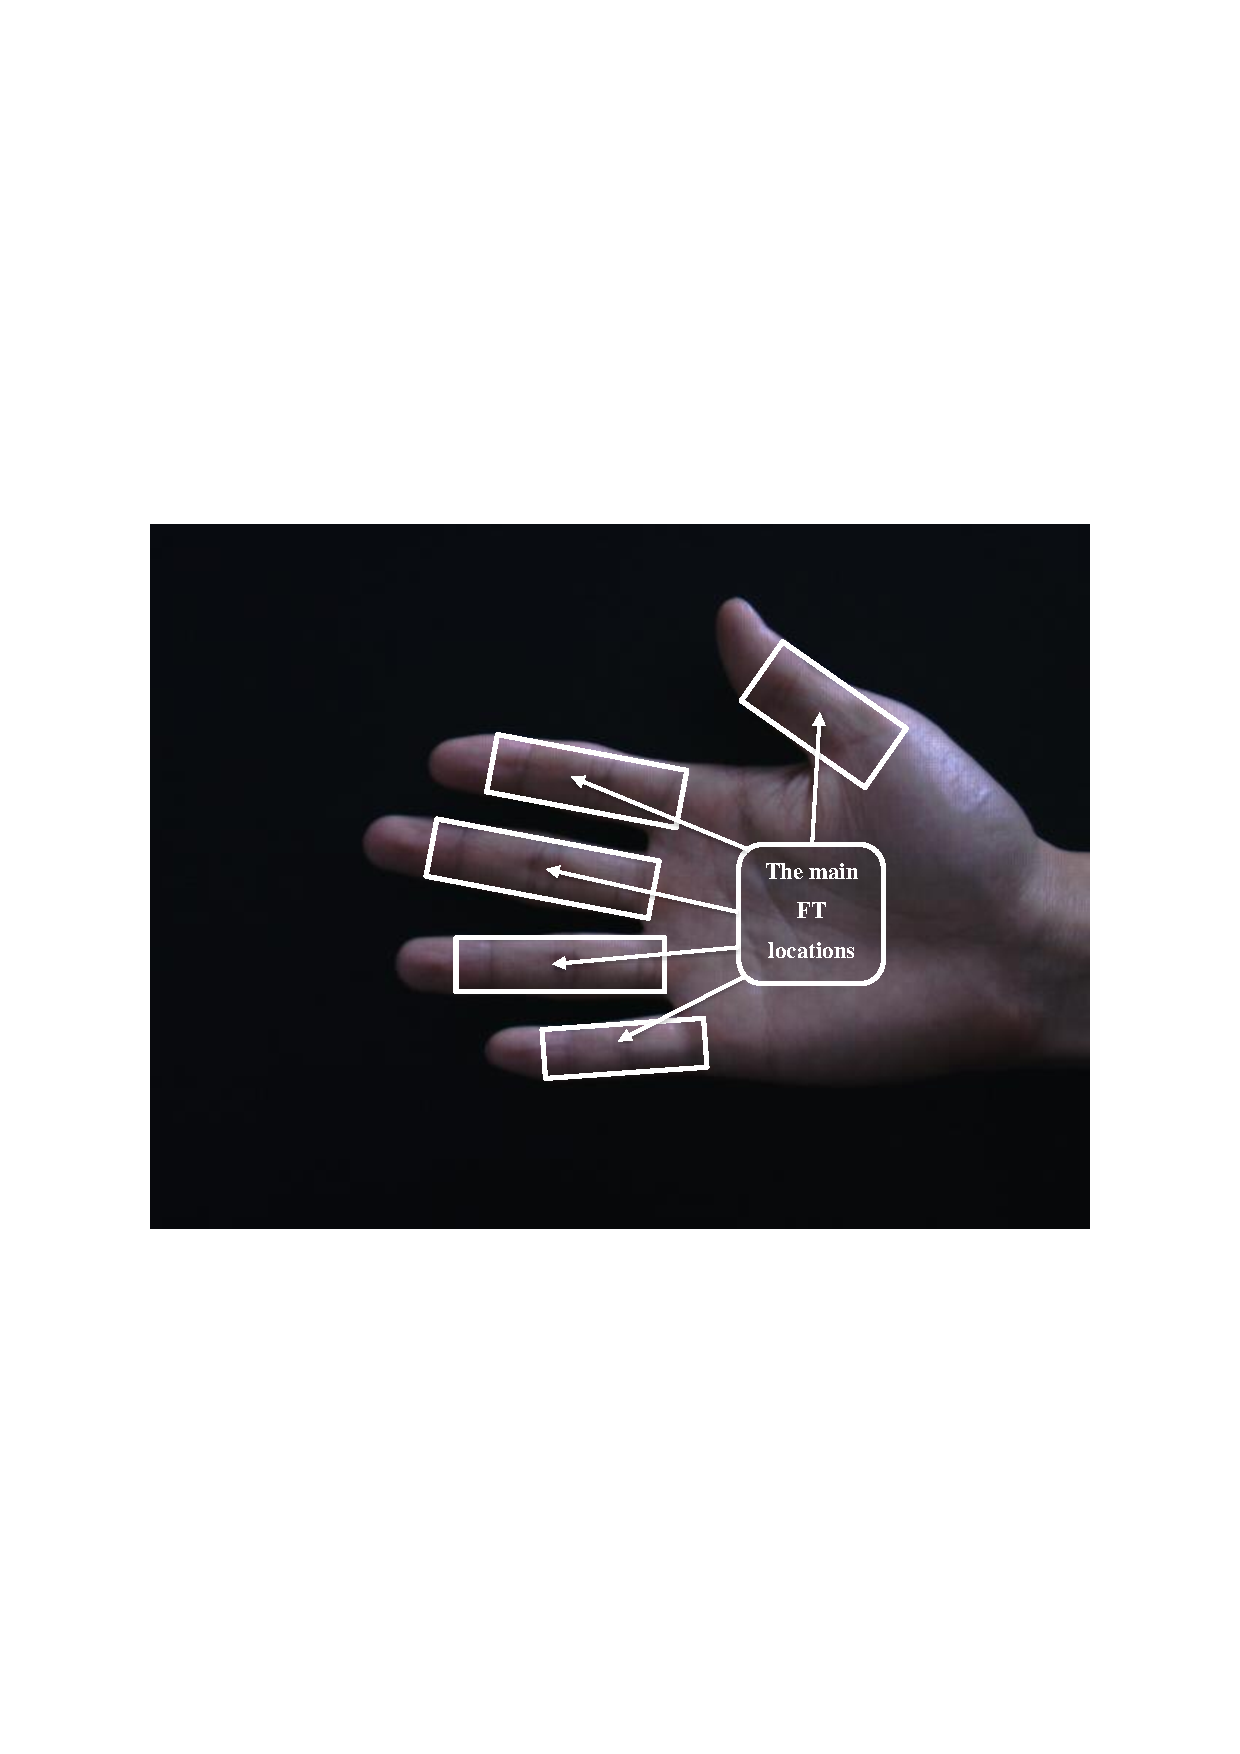
\includegraphics[page=1,scale=.5,trim=3cm 9cm 3cm 9cm,clip]{FT_locations_patterns.pdf}
    \caption{The main FT locations in the five fingers (little, ring, middle, index and thumb)}
    \label{fig:FT_locations}
\end{figure}\\
The aim of this paper is to enhance the verification accuracy and performance by suggesting the Deep Finger Texture Learning (DFTL) approach. The main contribution of this paper is to apply the deep learning technique to finger texture recognition to verify people faster and more accurately. This work overcame some FT verification drawbacks, which can be observed in recent studies, such as applying multiple processing stages, employing big neural network architectures, using large memory sizes and exploiting all the fingers to achieve the best performance.

The rest of this paper is organized as follows: Section II presents the related prior work. Section III explains the methodology of the work. Section IV discusses the results. Finally, Section V illustrates the conclusion.
%\begin{figure}[h]
%    \centering
%    \begin{subfigure}[b]{0.4\textwidth}
%    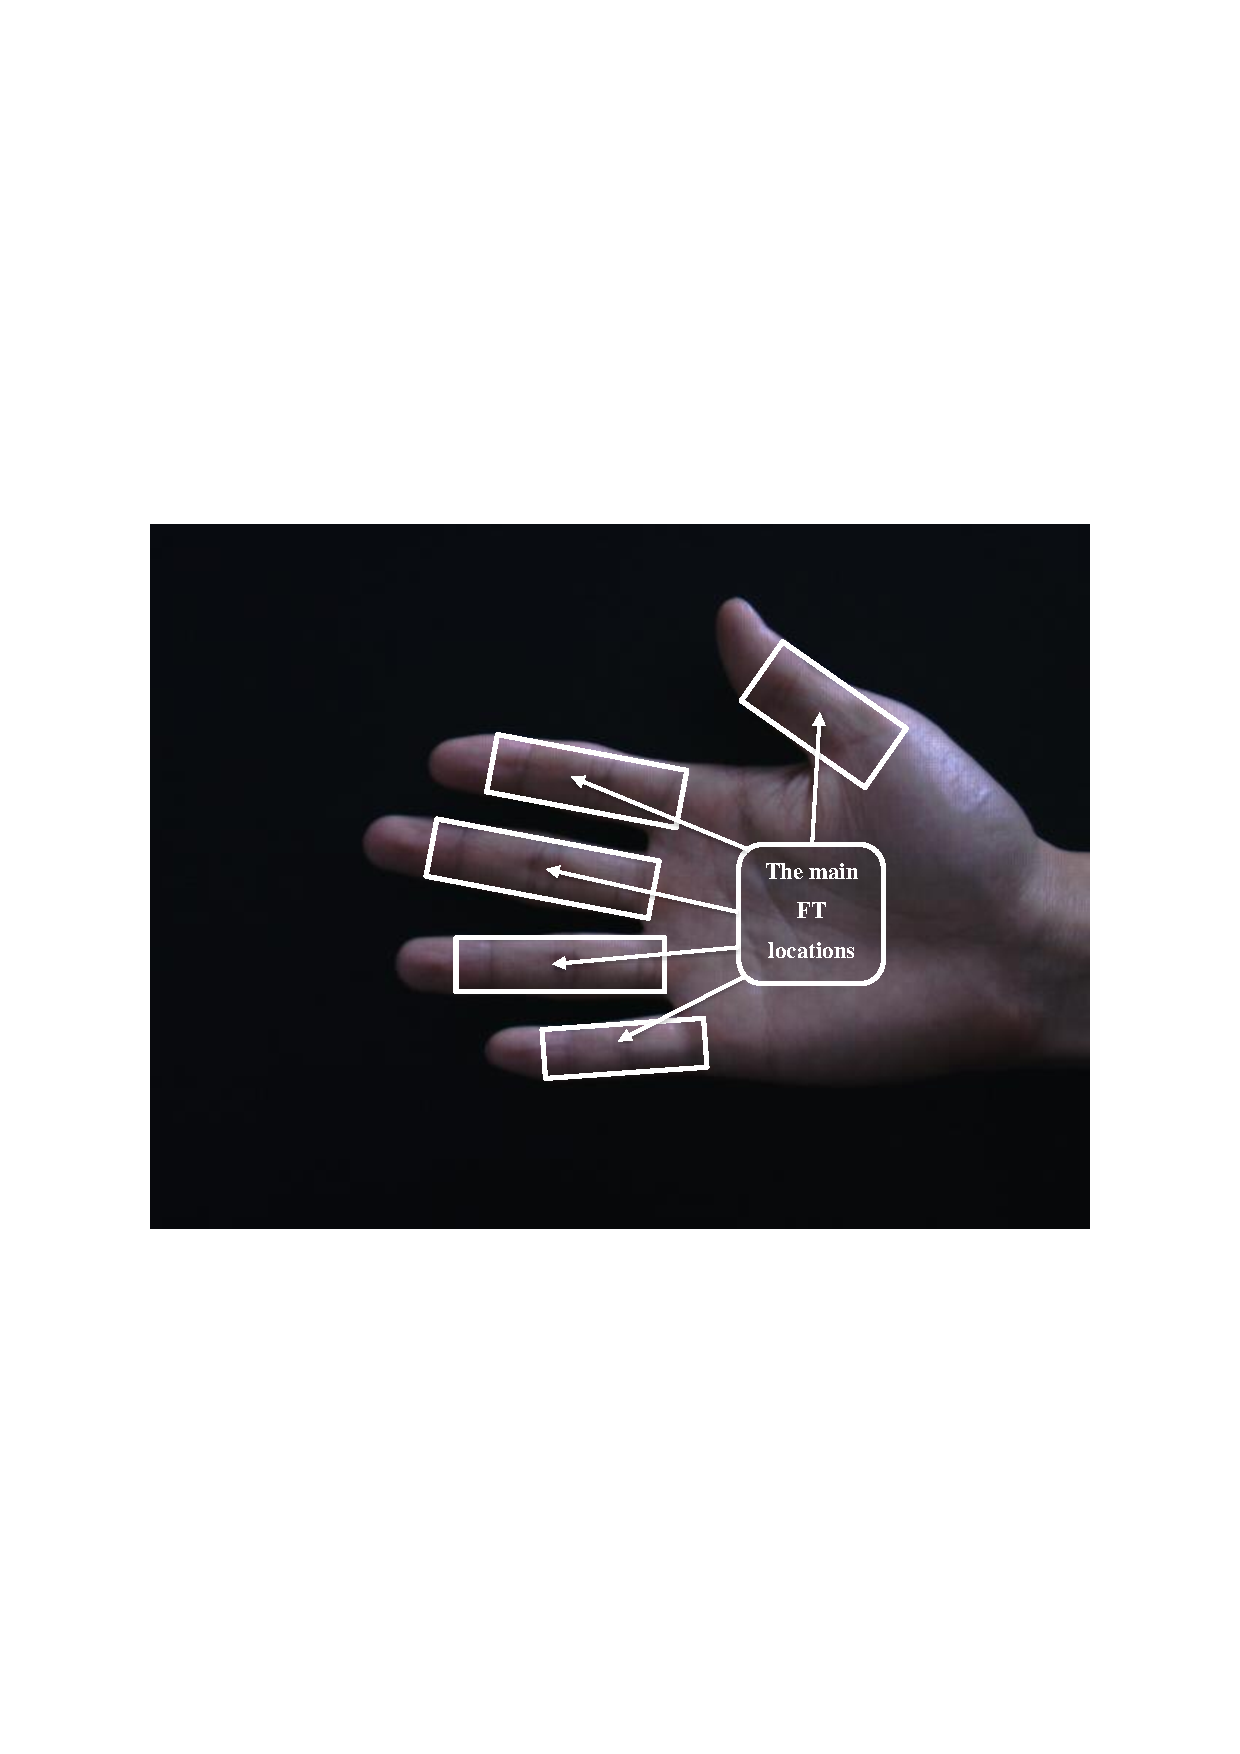
\includegraphics[page=1,scale=.5,trim=3cm 8cm 3cm 8cm,clip]{FT_locations_patterns.pdf}
%    \caption{}
%	\end{subfigure}
%    \centering
%    \begin{subfigure}[b]{0.4\textwidth}
%    \includegraphics[page=2,scale=.5,trim=3cm 11cm 3cm 10cm,clip]{FT_locations_patterns.pdf}
%    \caption{}
%	\end{subfigure}
%	\label{fig:FT_locations_patterns}
%	\caption{The main FT locations and components:\\
%	(a) The main FT locations.\\
%	(b) The main FT components.}
%\end{figure} \\ 

\section{Prior Work}
\begin{figure*}[!t]
    \centering
    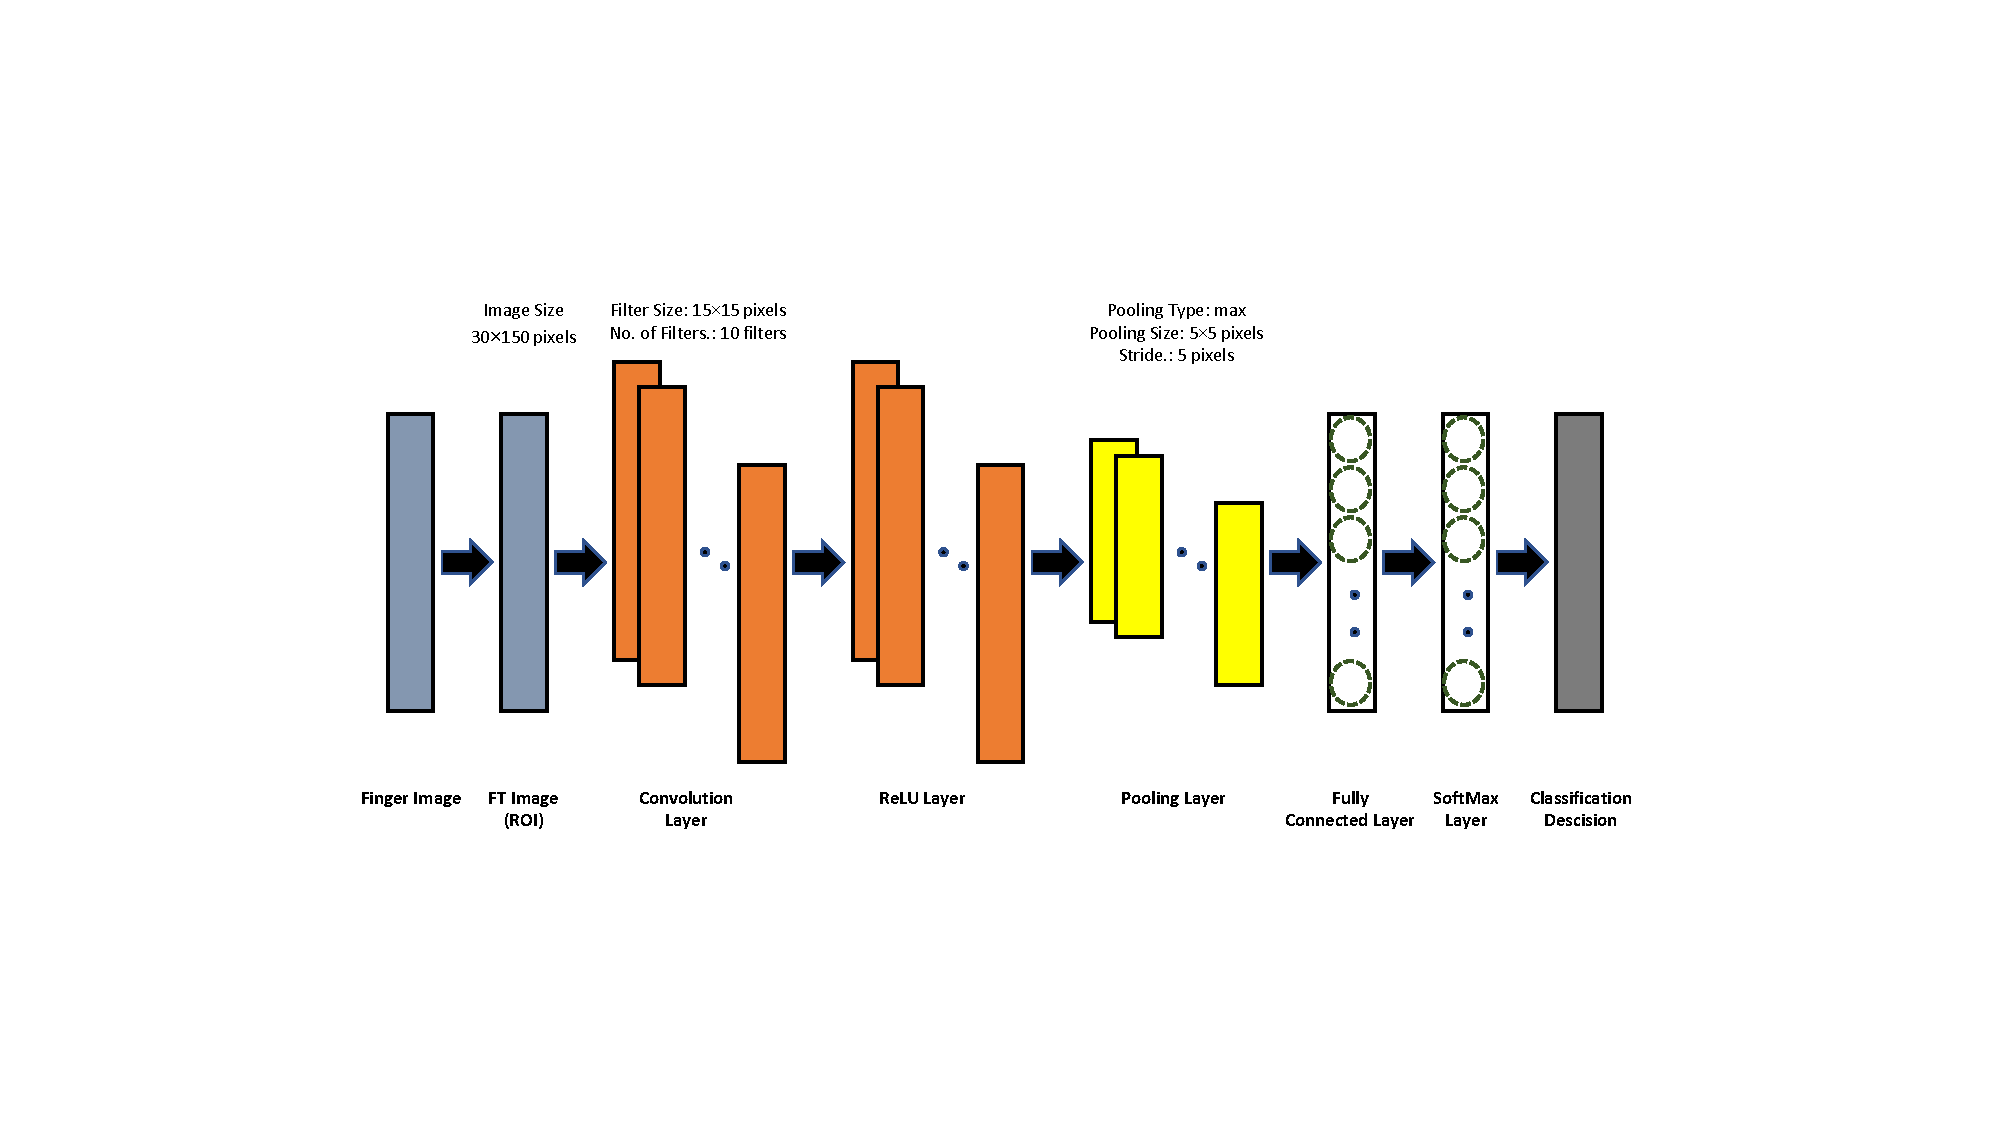
\includegraphics[page=1,height=7cm,width=20cm,trim=5cm 4cm 3cm 4cm,clip]{DFTL.pdf}
    \caption{The proposed architecture of the DFTL, it only exploits main deep learning layers}
    \label{fig:DFTL}
\end{figure*}
The idea of exploiting the FT as a biometric characteristic has been started in 2005, where Ribaric and Fratric fused the FTs of five fingers with the palm print in the case of individual identification \cite{Ribaric2005ABiometric}. In 2009, Pavesic \textit{et al.} combined the FTs of four fingers (little, ring, middle and index) with their fingerprints to establish a comparison study between different feature extraction methods \cite{Pavesic2009Finger-based}. In 2011, Kanhangad \textit{et al.} also utilized the FTs as a part of their study, where the authors fused the FTs with different hand characteristics to enhance the recognition \cite{Kanhangad2011AUnified}. In 2014, Bhaskar and Veluchamy described multiple biometric system by using a combination between palm print features and FTs features \cite{Bhaskar2014Hand}. 

In 2015, Al-Nima \textit{et al.} investigated employing the full FT regions of four fingers to enhance the verification performance. Concatenations between extracted FT features with the Probabilistic Neural Network (PNN) were applied to confirm the outcomes \cite{Al-Nima2015Human}. Thus, the main regions of the FTs for the four fingers were specified in that work. In 2017, Al-Nima \textit{et al.} expanded the FT study to suggest a robust finger segmentation approach, enhance a feature extraction method and introduce a novel approach to salvage the missing FT features \cite{Al-Nima2017Robust}. In 2017, Al-Nima \textit{et al.} proposed another finger segmentation approach to collect the finger images from different hand postures. Consequently, extracted the Region of Interests (ROIs) of the five FTs \cite{Al-Nima2017efficient}. Also in 2017, Al-Nima \textit{et al.} explained a new FT feature extraction method called the Multi-scale Sobel Angles Local Binary Pattern (MSALBP) and described an innovation combination classifier named the Finger Contribution Fusion Neural Network (FCFNN) in terms of personal verification \cite{Al-Nima2017finger}. 

It can be investigated from the prior FT studies that the deep learning did not employ to this phenomenon, although a large number of FT images were provided. In addition, previous FT characteristic publications had to apply multiple processes in the case of personal recognition. Usually, best FT feature extraction methods consist of different stages to analyse the vertical and horizontal patterns, then, extracting the features from the resulted values as in \cite{Al-Nima2017Robust} \cite{Al-Nima2017finger} \cite{Al-Nima2017efficient}. Data arrangements are always performed to justify the variances between different sample information, for example, applying data windowing and statistical computations \cite{Al-Nima2015Human} \cite{Al-Nima2016ANovel}. The determined classifier is commonly selected under the requirements of managing and fusing various data, for instance, combining the FT features of four or five fingers as in \cite{Pavesic2009Finger-based} \cite{Kanhangad2011AUnified} \cite{Al-Nima2017Robust} \cite{Al-Nima2017finger}. As a result, the classifier is often constructed by a big architecture. \marginpar{What does this mean?}

This study can reduce the number of operations and enhance the FT performance in the case of human verification. 
%Comparisons with recent work have been established.

\section{Methodology}
In this section the theoretical structure of the Deep Finger Texture Learning (DFTL) approach will be described. 

As mentioned, extensive studies were introduced to collect the FT features, employ statistical computations and apply a beneficial classifier with investigating an appropriate combination scheme. The suggested DFTL has less complicated yet effective architecture. Fig. \ref{fig:DFTL} depicts the proposed DFTL.

It can be seen that the DFTL only exploits main deep learning layers (convolution, ReLU, pooling, fully connected and SoftMax), where each one of these layers does not need to be repeated as in the convolutional neural network. This is due to the analysing requirements of the FT patterns, where the FT patterns have simple descriptions of horizontal and vertical patterns. Therefore, to justify these patterns simple stages can be used in a deep learning network. \marginpar{From here on: How does the large number of images guarantee the applicability of deep learning?}It is worth mentioning that it is applicable to use the deep learning with the FT images. This is because of the capability of collecting a large number of samples. To explain, each single hand contains five FT samples, so, by increasing the number of acquired hand images this dramatically increases the number of FT images. 

In the following, we will explain how it works in each layer.

\subsection{Finger Segmentation and FT Region Extraction}
The DFTL structure starts from the finger segmentation. This has been achieved by applying the finger segmentation method in \cite{Al-Nima2017Robust}. After that, extracting the ROI of the FT has been performed according to the Adaptive Inner Rectangle (AIR), which has been modified in \cite{Al-Nima2017Robust} and \cite{Al-Nima2017efficient}. Each FT image is resized to $30 \times 150$ pixels as this size can provide fair comparisons with prior studies.

\subsection{Convolution Layer}
One convolution layer is used. Empirically, this has been found to be sufficient, because the FTs consist of simple patterns. In this layer, the FT input image $\textbf{X}$ will be analysed into a feature map. The feature map is denoted as a convolution with a kernel weight of channel $C$, which is here equal to 1 as we are using one channel of grayscale FT images. \marginpar{Does it mean that there is only one channel?} In general, this kernel has a size of $k_h \times k_w \times C$ followed by the addition of bias. Note that $k_h$ is ... and $k_w$ is ...\marginpar{Fix here.} Let $W_{i,j,c^{l-1}}^{c^{l}}$ be the components of the kernel weights, $B_{c^{l}}$ represents the channel bias of the convolution layer, $l-1$ represents the previous layer and $l$ represents the current layer. The value $z_{u,v,c^{l}}$ of an assigned pixel at $(u,v)$ in channel $c^{l}$ of the layer $l$ is given by:
\begin{equation}
z_{u,v,c^{l}}= \text{\footnotesize $B_{c^{l}}+\sum_{i=-k_h^{l}}^{k_h^{l}}\sum_{j=-k_w^{l}}^{k_w^{l}}\sum_{c^{l-1}=1}^{C^{l-1}} W_{i+k_h^{l},j+k_w^{l},c^{l-1}}^{c^{l}} z_{u+i,v+j,c^{l-1}}$}
\label{eq:conv_layer}
\end{equation}
where $z_{u,v,c^{l}}$ represents the outcome of a convolution layer node, $k_h^{l}=(k_h-1)/2$ and $k_w^{l}=(k_w-1)/2$ \cite{simo2016learning}. \marginpar{Does it mean that all the $k_w^l$ are the same for all layers?}
%Again, this layer analyses the input values and produces FTs' feature maps.

\subsection{ReLU Layer}
Subsequently, a Rectified Linear Unit (ReLU) activation function is applied in the ReLU layer. This layer has an advantage of providing non-linear computations to the DFTL. It removes the negative values and preserves the positive values from a feature map. Equation (\ref{eq:relu_layer}) is utilized to perform the ReLU activation function:
\begin{equation}
o_{u,v,c^{l}}=f(z_{u,v,c^{l}})=\max(0,z_{u,v,c^{l}})
\label{eq:relu_layer}
\end{equation}
where $o_{u,v,c^{l}}$ represents the outcome of a ReLU layer node and $\max$ represents the maximum operation \cite{krizhevsky2012imagenet}.\\

\subsection{Pooling Layer}
Hereafter, a pooling layer is employed to reduce the feature map size. In general, the pooling layer can be implemented according to the following equation:
\begin{equation}
q_{a^{l},b^{l},c}=\underset{0\leq a<p_h,0\leq b<p_w}{\max} o_{a^{l}\times p_h+a, b^{l}\times p_w+b,c}
\label{eq:pooling_layer}
\end{equation}
where $q_{a^{l},b^{l},c}$ represents the outcome of a pooling layer node, $0\leq a^{l} <p_h^{l}$, $p_h^{l}$ represents the height of the pooled feature map, $0\leq b^{l} <p_w^{l}$, $p_w^{l}$ represents the width of the pooled feature map, $0\leq c <C^{l}=C^{l-1}$, $p_h$ and $p_w$ respectively represent the height and width of the feature map subregions that need to be pooled \cite{wu2017introduction}. 

\subsection{Fully Connected Layer}
Now, fully connected layer is applied to map between the pooling layer and the required number of recognizing subjects. Equation (\ref{eq:fully_connect}) simulates the operation of the fully connected layer. The produced feature maps in layer $l-1$ are interpreted as $m_1^{l-1} \times m_2^{l-1} \times m_3^{l-1}$ dimensional vectors as follows:
\begin{equation}
g_{r}=\text{\footnotesize $\sum_{a=1}^{m_1^{l-1}} \sum_{b=1}^{m_2^{l-1}} \sum_{c=1}^{m_3^{l-1}} W_{a,b,c,r}^{l}(\textit{\textbf{Q}}_{c})_{a,b}~, ~~~~~~~\forall 1 \leq r \leq m^{l}$}
\label{eq:fully_connect}
\end{equation}
where $g_{r}$ represents the outcome of a fully connected layer node, $m_1^{l-1}$ represents the height of a feature map in the previous layer $l-1$, $m_2^{l-1}$ represents the width of a feature map in the previous layer, $m_3^{l-1}$ represents the number of generated feature maps in the previous layer, $W_{a,b,c,r}^{l}$ represents the connection weights between the pooling layer and the fully connected layer, and $m^{l}$ represents the number of required recognizing subjects \cite{stutz2014neural}.\marginpar{What is $\textit{\textbf{Q}}$?}

\subsection{Softmax Layer}
Consequently, softmax activation function can be used to compute posterior classification probabilities. It utilizes the following equation:
\begin{equation}
y_{r}=\frac{\exp(g_{r})}{\sum_{s=1}^{m^{l-1}}\exp(g_{s})} 
\label{eq:softmax}
\end{equation}
where $y_{r}^{(l)}$ represents the outcome of a softmax layer node \cite{stutz2014neural}.

\subsection{Classification Layer}
Finally, to achieve the final decision, a classification layer is used. This layer follows a competitive rule called the winner-takes-all rule. \\
The operation in this layer can be described in Equation (\ref{decision}): \\
\begin{equation}
D_{r}=\left\{\begin{matrix}
1 & $if$~y_{r}=max \\ 
0 &  $otherwise$
\end{matrix}\right.
,~~~r=1,2,...,class
\label{decision}
\end{equation}\\
where $D_{r}$ represents the output decision of a classification layer node and $max$ represents the extracted maximum $y_{r}$ value \cite{Al-Nima2017Signal}.\\
Due to the fact that a multi-class classifier can be utilized for verifying subjects \cite{Al-Nima2015Human} \cite{Al-Nima2017finger}, we have adapted the DFTL for the human verification by using its multi-class outputs of the classification layer.

\section{Results and Discussions}
\subsection{Descriptions of Employed Databases}
Four databases with large numbers of contactless hand images have been employed in this paper. The first database is from the Hong Kong Polytechnic University Contact-free 3D/2D (PolyU2D) Hand Images Database (Version 1.0) \cite{Databasever1PolyU3D2D}. It consists of 8,850 fingers from 1770 very low resolution hand images. The second database is from the Indian Institute of Technology Delhi (IITD) Palmprint Image Database (Version 1.0). The participants of this database were asked to provide high degrees of hand movements during the capturing step \cite{IIT-Delhi-PalmprintV1} \cite{kumar2008incorporating}. A total of 4,440 finger images have been used in this study. They have been collected from 888 high resolution hand images. The third database is for a specific spectral wavelength of 460nm (or blue light), which can be found in the CASIA Multi-Spectral Palmprint image database (Version 1.0) \cite{CASIAMS-PalmprintV1}. This data contains FT features as mentioned in \cite{Khan2011Contour}\cite{khan2014multispectral}. It has 3,000 fingers included in 600 low resolution hand images. It is valuable to work with this type of database as it has different FT features than that acquired under the normal light. In this paper, we will refer to this database by CASIA-BLU. The fourth database is for a white spectral (or white light), which can be also found in the CASIA Multi-Spectral Palmprint image database (Version 1.0) \cite{CASIAMS-PalmprintV1}. This data contains standard FT features as it collected under a white light. It has the same number of samples as in CASIA-BLU. In this paper, we will refer to this database by CASIA-WHT. 

\subsection{Practical Experiments}
The following process has been implemented to 2D right hand images of all the employed databases: 25 finger images for each person or subject have been utilized in the training phase following \cite{Al-Nima2017Robust} \cite{Al-Nima2017efficient} \cite{Al-Nima2017finger}; the remaining samples have been used in the testing phase. All the five finger images (thumb, index, middle, ring and little) have been considered in this paper. However, any finger can confirm the personal verification in the DFTL.\\
The ROIs of the five finger images have been extracted according to \cite{Al-Nima2017Robust} \cite{Al-Nima2017finger}, where the image resizing is equally normalized to $30\times 150$ pixels. By employing similar FT normalizations, fair comparisons can be established. \\
%\begin{figure}[!h]
%    \centering
%    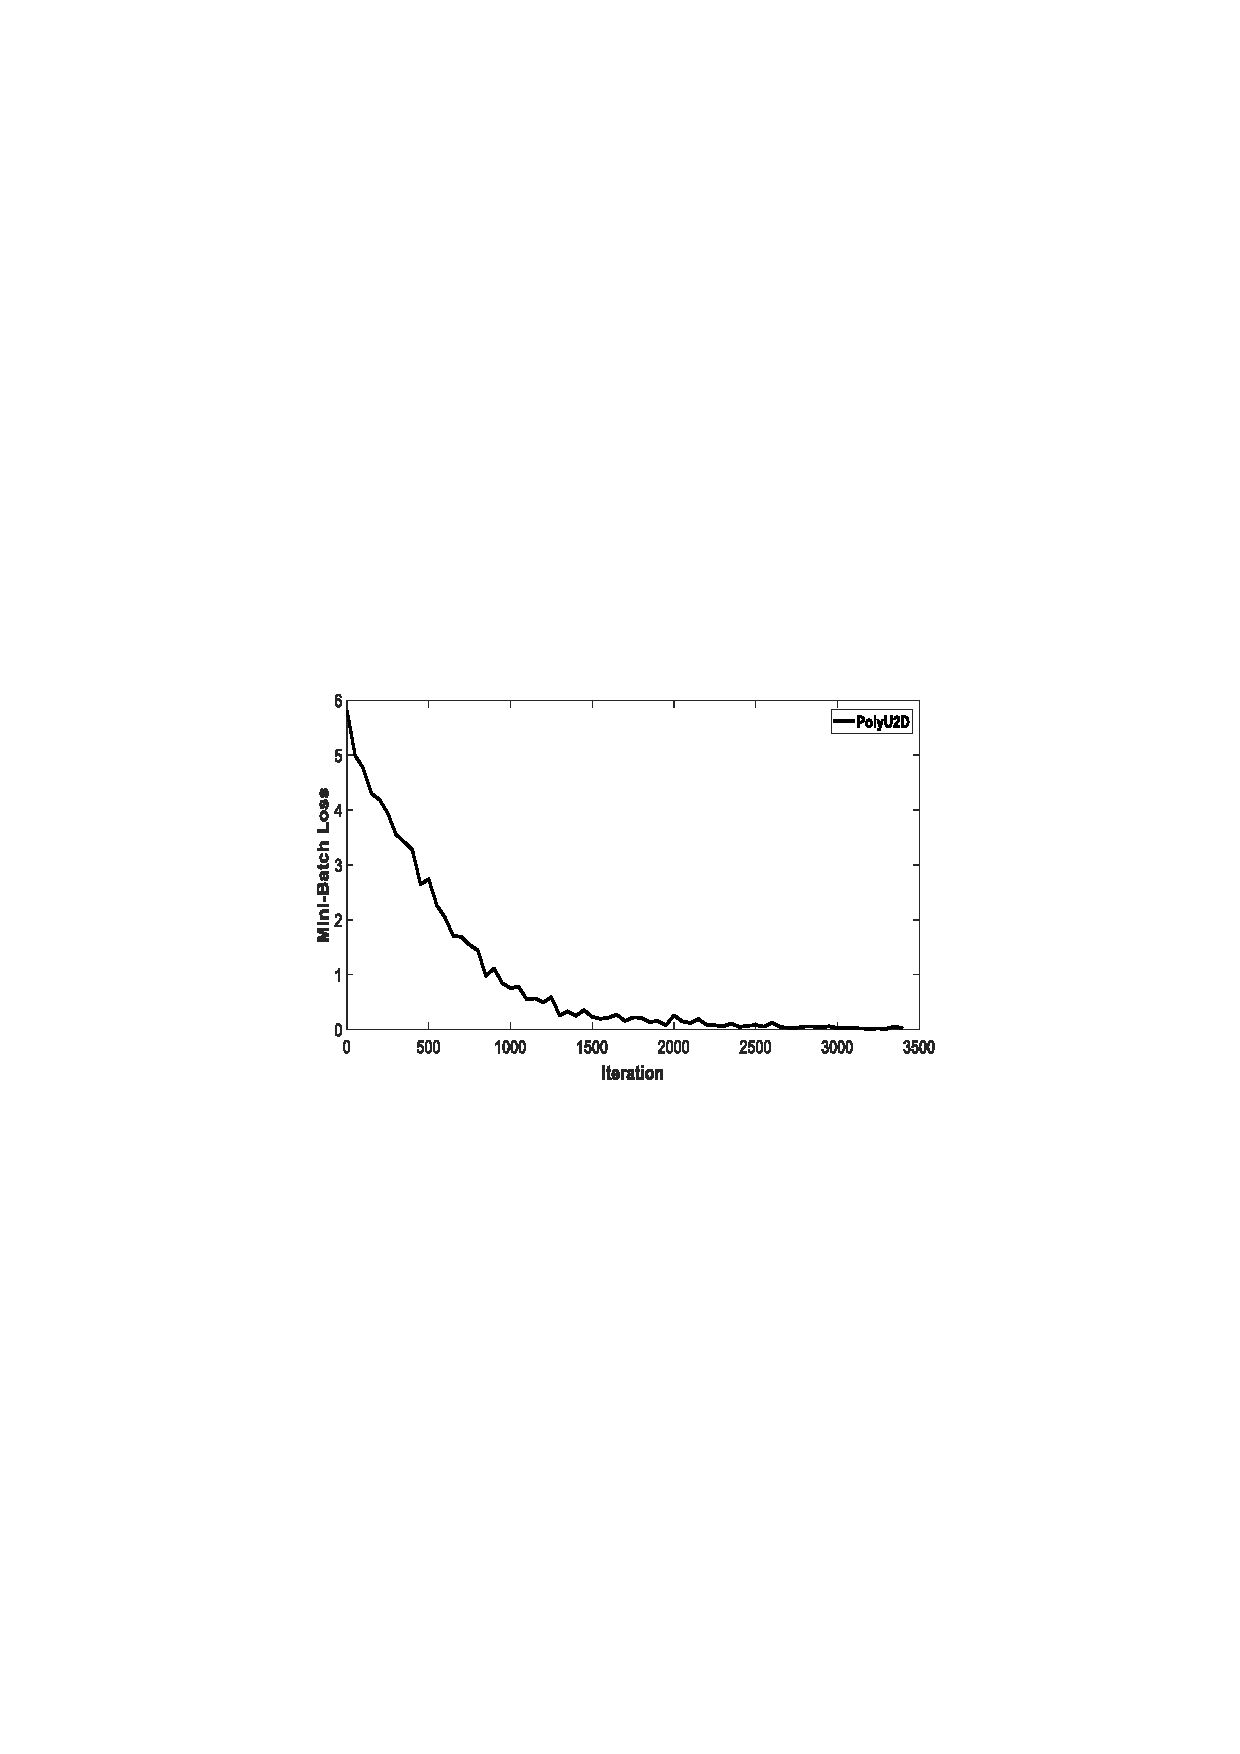
\includegraphics[page=1,scale=.8,trim=5cm 11.25cm 5cm 11.25cm,clip]{Iteration_vs_Loss_PolyU2D.pdf}
%    \caption{PolyU2D training curve}
%    \label{fig:PolyU2D_training_curve}
%\end{figure}
%\begin{figure}[!h]
%    \centering
%    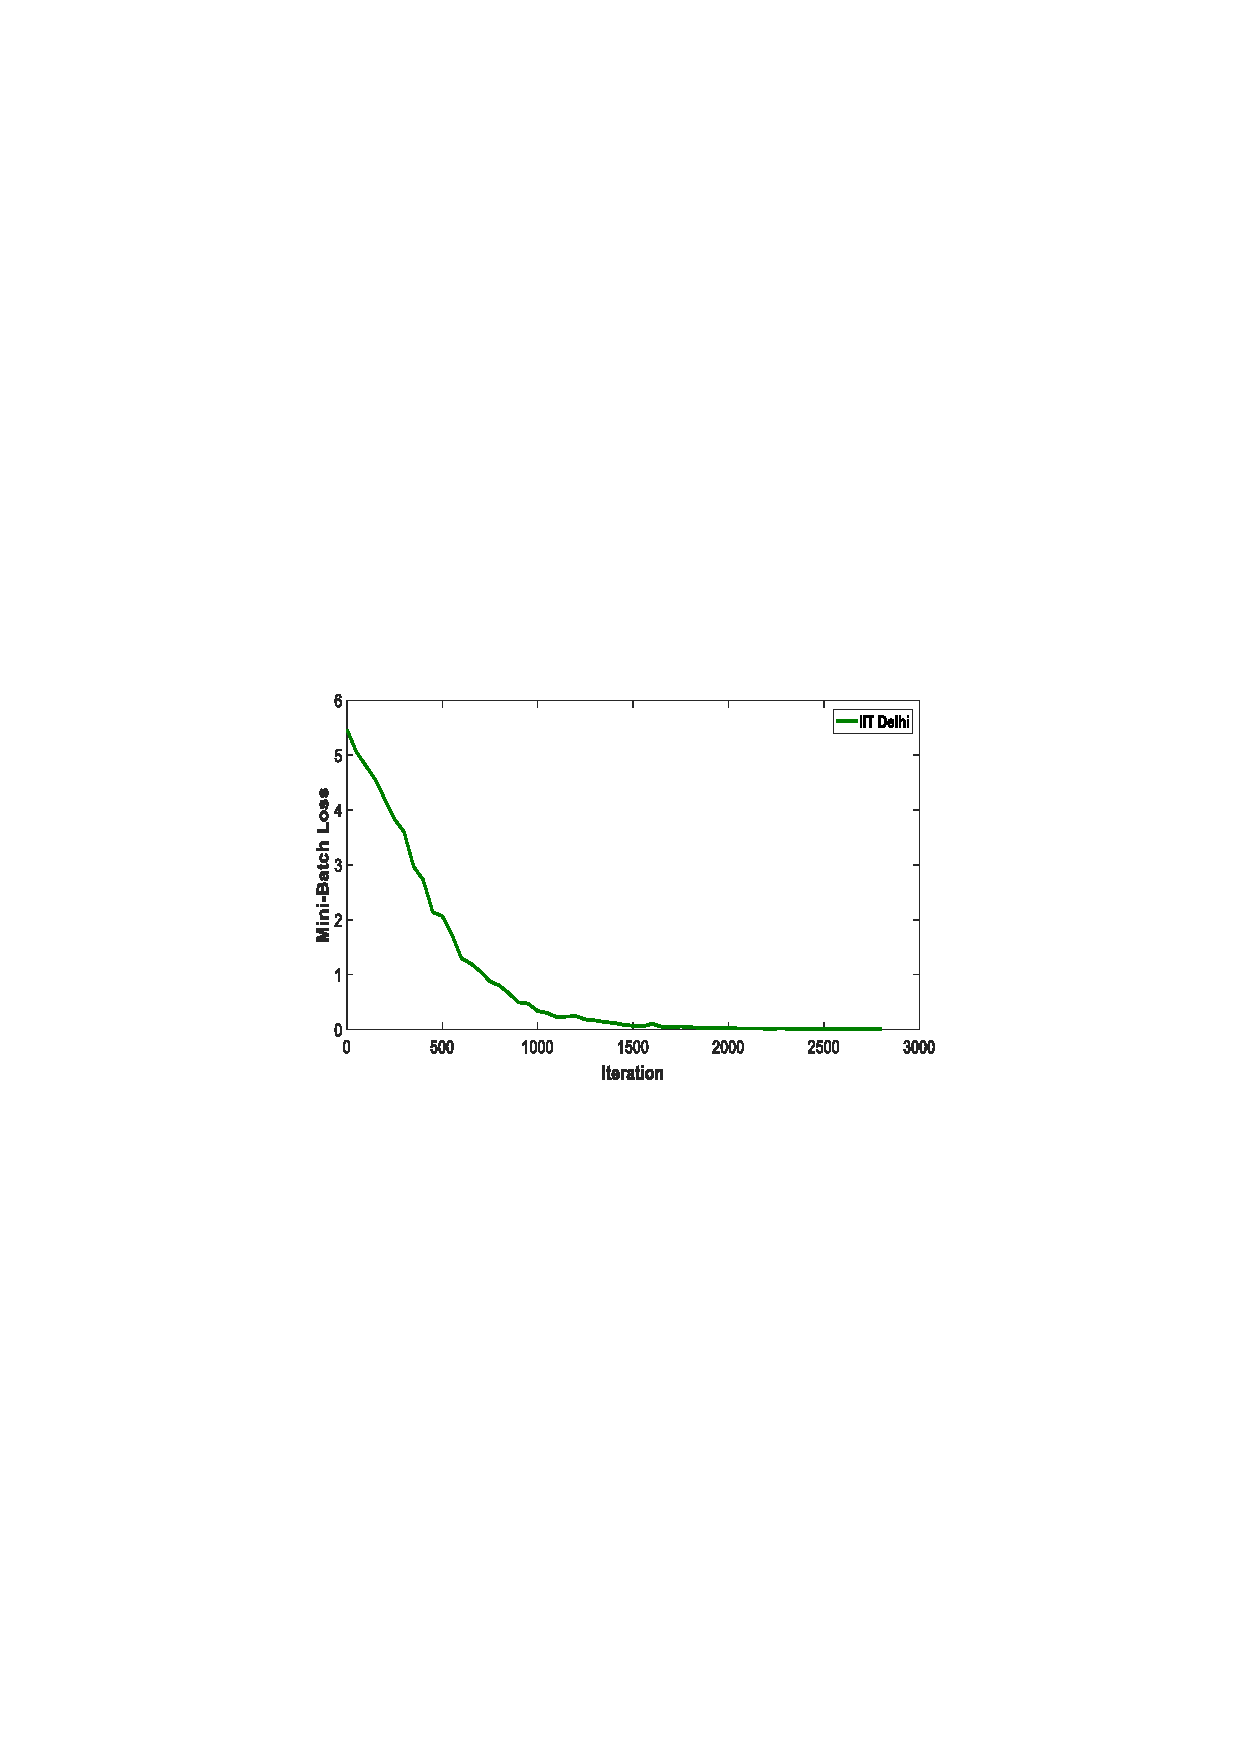
\includegraphics[page=1,scale=.8,trim=5cm 11.25cm 5cm 10.8cm,clip]{Iteration_vs_Loss_IIT.pdf}
%    \caption{IIT training curve}
%    \label{fig:IIT_training_curve}
%\end{figure}
%\begin{figure}[!h]
%    \centering
%    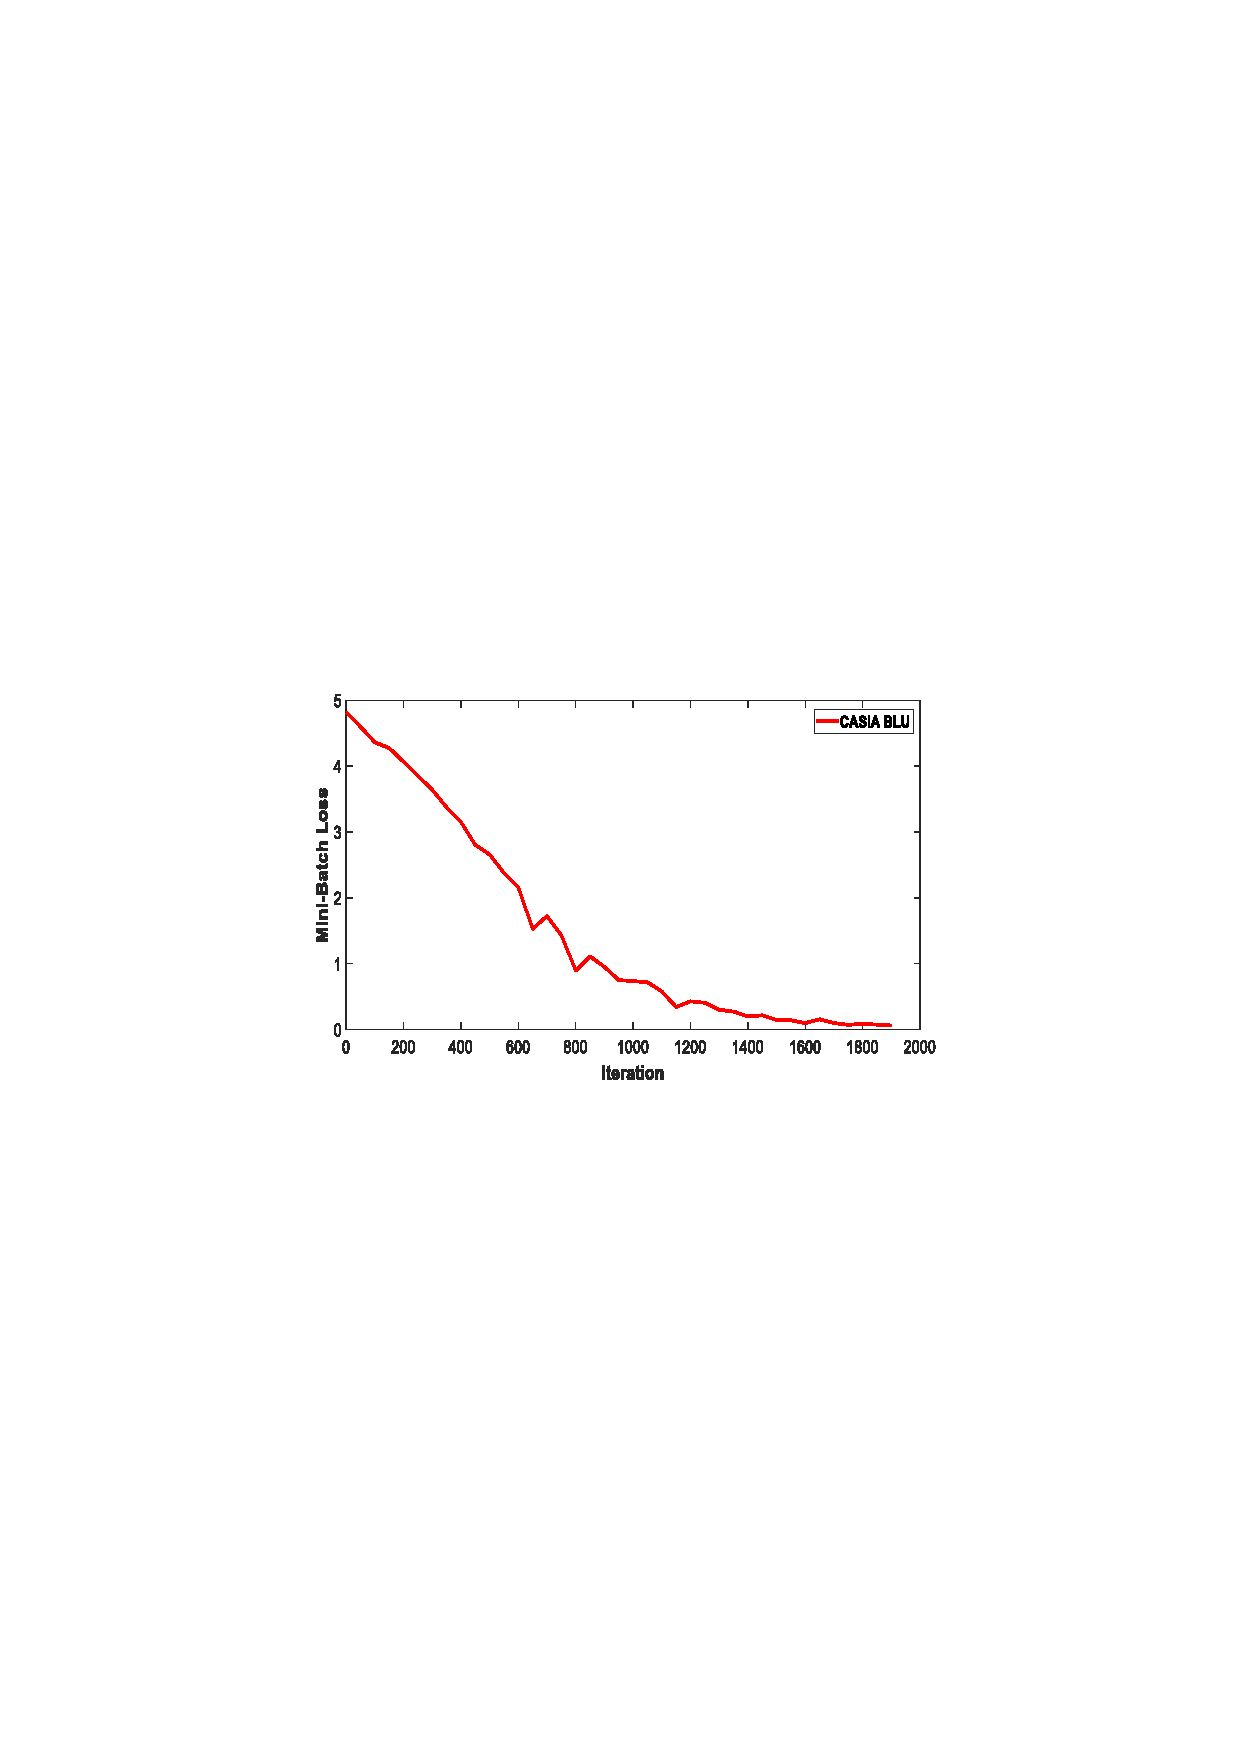
\includegraphics[page=1,scale=.8,trim=5cm 11.25cm 5cm 11.25cm,clip]{Iteration_vs_Loss_CASIA_BLU.pdf}
%    \caption{CASIA-BLU training curve}
%    \label{fig:CASIA-BLU_training_curve}
%\end{figure}
%\begin{figure}[!t]
%    \centering
%    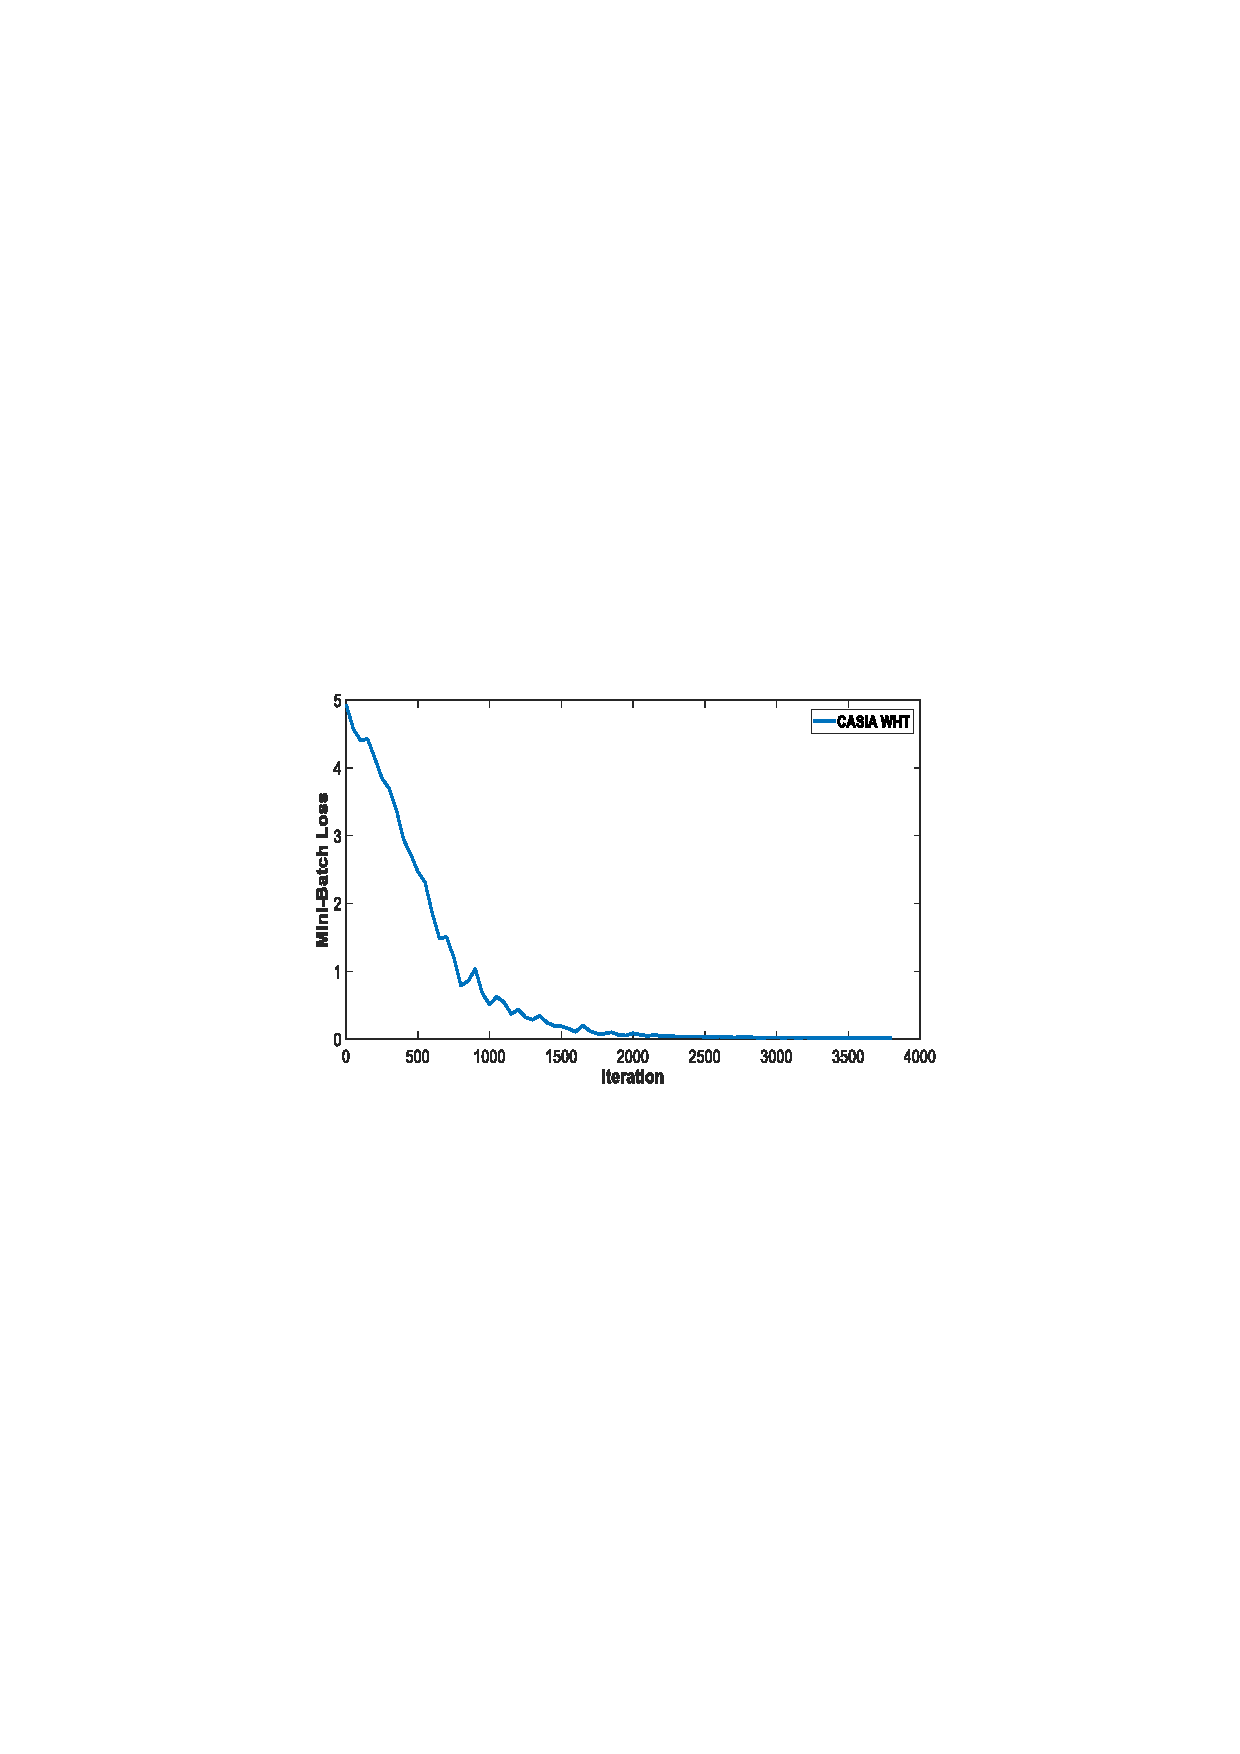
\includegraphics[page=1,scale=.8,trim=5cm 11.25cm 5cm 11.25cm,clip]{Iteration_vs_Loss_CASIA_WHT.pdf}
%    \caption{CASIA-WHT training curve}
%    \label{fig:CASIA-WHT_training_curve}
%\end{figure}
The output of the DFTL is aimed to generate the verification decision, where each neuron in the last layer refers to a person. The number of output values is equal to the number of the output neurons and this is equal to the number of utilized subjects. This means that 177, 148, 100 and 100 output neurons have been assigned for the PolyU2D, IITD, CASIA-BLU and CASIA-WHT databases, respectively. \\
First of all, the suggested DFTL network has been trained for each set of FTs in each database. Fig. \ref{fig:Training_curves} indicates the success of the training phases for the four databases. It illustrates the relationships between the iterations and the Mini-batches losses, where a mini-batch is defined in \cite{beale1992neural} as a training data sub-group and it utilizes to adjust the weights after assessing the gradient of the loss function. The loss function is denoted as the cross entropy loss function, which is the probability that the network assigns the class $r$ for the $e$th input $P(t_r=1|x_e)$ \cite{beale1992neural}.
\begin{figure}[!b]
    \centering
    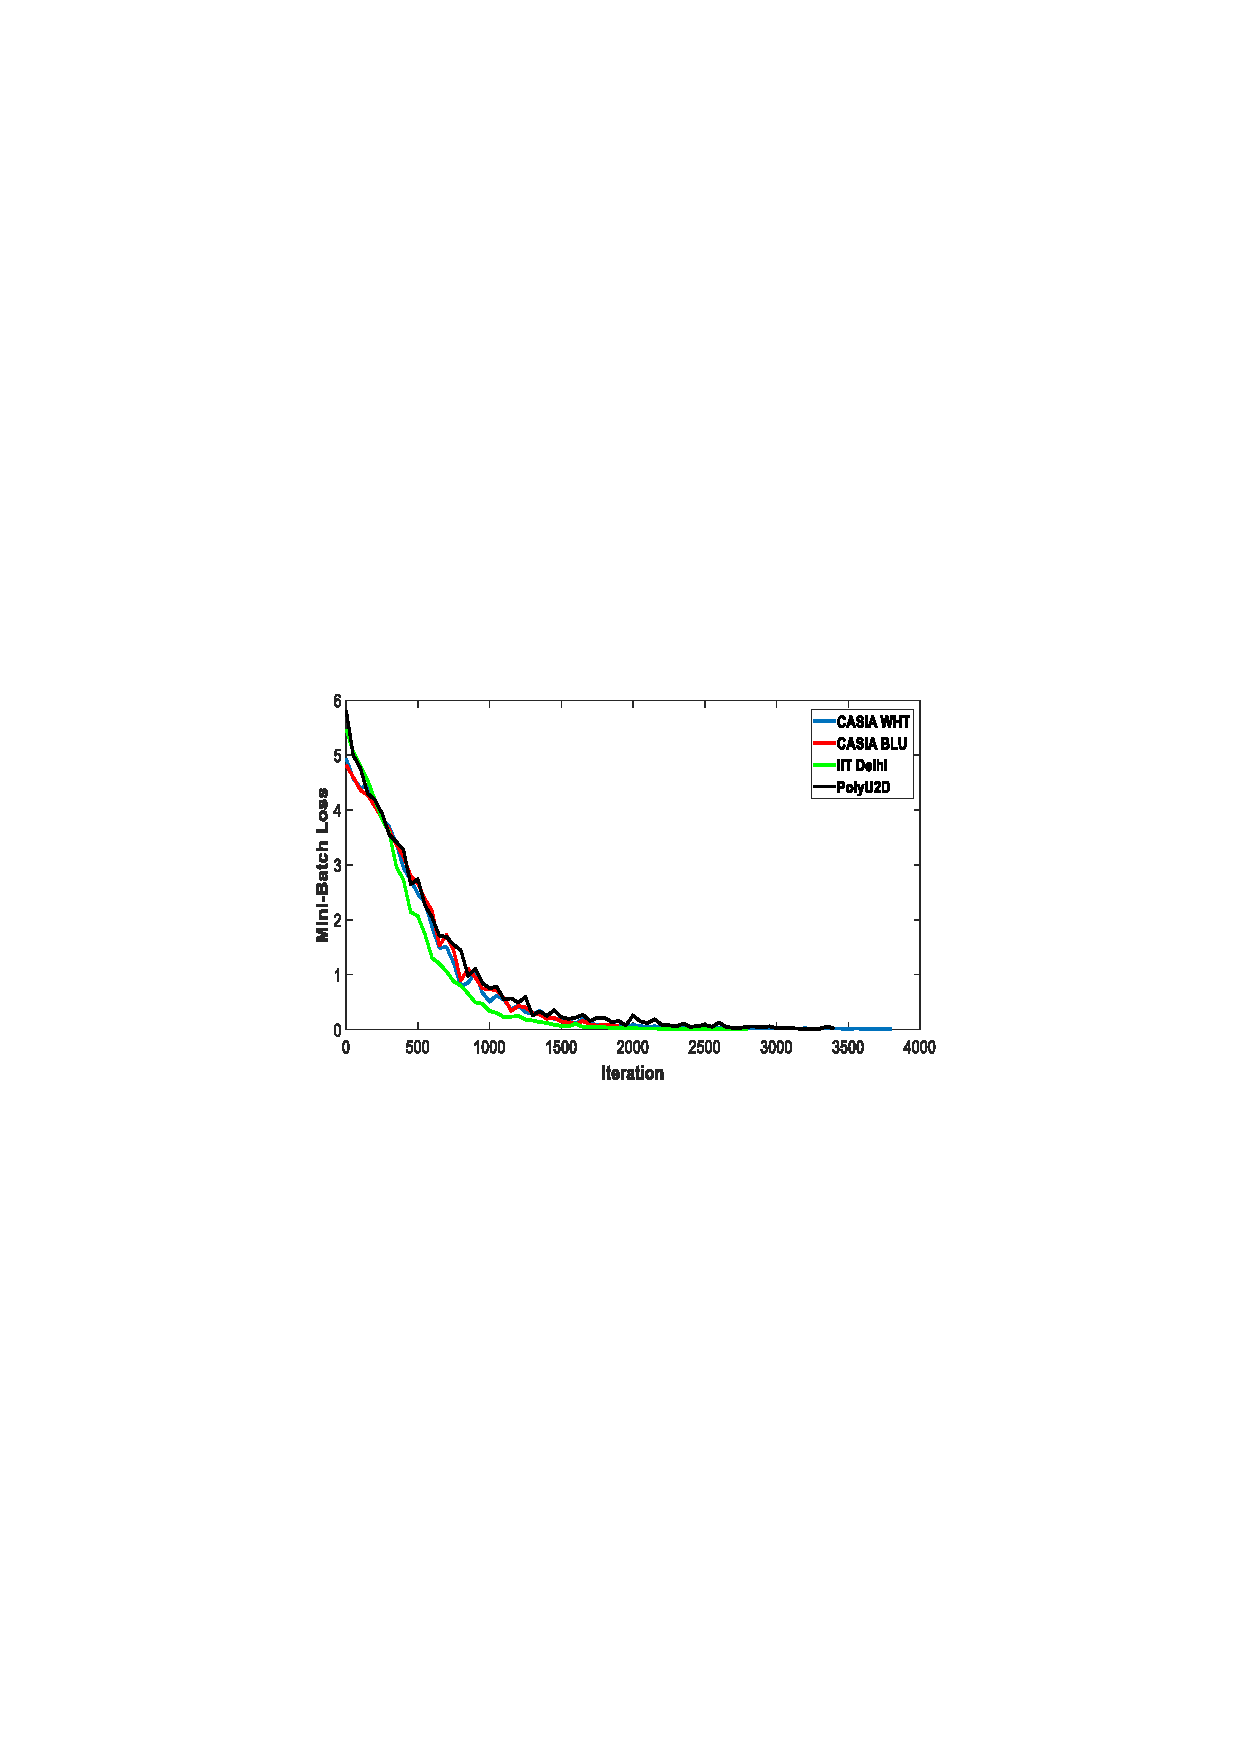
\includegraphics[page=1,scale=.8,trim=5cm 11.25cm 5cm 11.25cm,clip]{Iteration_vs_Loss_All_Databases.pdf}
    \caption{The relationships between the iterations and the mini-batches losses for the four employed databases during the training phases}
    \label{fig:Training_curves}
\end{figure}\\
The DFTL parameters have been established after many experiments. The filter size with the number of filters in the convolution layer have been found to be $15 \times 15$ pixels and 10 filters, respectively. In the pooling layer, the pooling type has been assigned to maximum numbers, where these numbers reserve the extracted features by the ReLU function. The pooling filter size with the stride have been determined to $5 \times 5$ pixels and 5 pixels, respectively. This is because that the pooling size filters and the stride parameters are respectively equivalent to the parameters of the windowing size and non-overlapped partitions in \cite{Al-Nima2015Human} \cite{Al-Nima2017Robust} \cite{Al-Nima2017efficient} \cite{Al-Nima2017finger}. Therefore, the same parameter settings have been determined, where they have been confirmed as the best selected parameters in \cite{Al-Nima2017Signal}.
\begin{table*}[]
\centering
\caption{The SVAs of different human verification methods by using the FT biometric characteristic}
\label{Table:SVA}
\begin{tabular}{|c|C{1.5cm}|C{1.5cm}|C{1.5cm}|C{1.5cm}|C{1.7cm}|C{1.7cm}|C{1.7cm}|C{1.7cm}|}
\hline
\multirow{3}{*}{\textbf{Reference}}  & \multicolumn{4}{c|}{\textbf{FT Recognition Process}} & \multicolumn{4}{c|}{\textbf{Databases}}\\ \cline{2-5} \cline{6-9}
& \textbf{\textit{Feature}}  &  \textbf{\textit{Windowing}} & \textbf{\textit{Statistical}} & \multirow{2}{*}{\textbf{\textit{Classifier}}} & \multirow{2}{*}{\textbf{\textit{PolyU2D}}} 
 & \multirow{2}{*}{\textbf{\textit{IITD}}} & \multirow{2}{*}{\textbf{\textit{CASIA-BLU}}} & \multirow{2}{*}{\textbf{\textit{CASIA-WHT}}} \\ 
 & \textbf{\textit{Extraction}} & \textbf{\textit{(pixels)}}&  \textbf{\textit{Calculations}} & & & & & \\ \hline
\cite{Al-Nima2015Human} &  IFE & $5 \times 5$ & COV & PNN & 98.53\% & --- & --- & --- \\ \hline
\cite{Al-Nima2017efficient} & LLBP \cite{Petpon2009Face}  & $5 \times 5$ & COV & PNN & 99.32\% & 97.97\% & 95\% & --- \\ \hline
\multirow{2}{*}{\cite{Al-Nima2017Robust}}  & ELLBP  & \multirow{2}{*}{$5 \times 5$} & \multirow{2}{*}{COV} & \multirow{2}{*}{PNN} & \multirow{2}{*}{99.66\%} & \multirow{2}{*}{98.65\%} & \multirow{2}{*}{97\%} & \multirow{2}{*}{---} \\ 
& (N=17)  & & & & &&& \\ \hline
\multirow{2}{*}{\cite{Al-Nima2017finger}} & MSALBP& \multirow{2}{*}{$5 \times 5$} & \multirow{2}{*}{COV} & \multirow{2}{*}{PNN} &\multirow{2}{*}{99.32\%} & \multirow{2}{*}{---} & \multirow{2}{*}{98\%} & \multirow{2}{*}{---} \\ 
 & (P=8,R=2)  & & & & &&& \\ \hline
\multirow{2}{*}{\cite{Al-Nima2017finger}} & MSALBP  & \multirow{2}{*}{$5 \times 5$} & \multirow{2}{*}{COV} & \multirow{2}{*}{FCFNN} & \multirow{2}{*}{99.77\%} & \multirow{2}{*}{---} & \multirow{2}{*}{98\%} & \multirow{2}{*}{---} \\ 
 & (P=8,R=2)  & & & & &&& \\ \hline
Our & \multicolumn{4}{c|}{\multirow{2}{*}{\textbf{DFTL}}}  & \multirow{2}{*}{\textbf{100\%}} & \multirow{2}{*}{\textbf{98.65\%}} & \multirow{2}{*}{\textbf{100\%}} & \multirow{2}{*}{\textbf{98\%}} \\ 
Approach & \multicolumn{4}{c|}{}  & &&& \\ \hline
\end{tabular}
\end{table*}
\\
The number of the successfully verified subjects has been counted and recorded for various verification methods based on the FT characteristic. The successful rates have been benchmarked as SVA values. Table \ref{Table:SVA} highlights a comparison between the outcomes of the different recognition methods. It can be observed that each of the prior FT studies used a determined feature extraction approach, non-overlapped windowing of $5 \times 5$ pixels, efficient statistical analysis computations called Coefficient of Variance (COV) and an effective classifier. As it can be seen from this table that the SVA \marginpar{What is SVA?} has been computed for the verification method in \cite{Al-Nima2015Human} and it attained 98.53\%. In that paper, large ROI sizes of the FTs and only four fingers in each hand image were applied for the PolyU2D database. Furthermore, an efficient feature extraction called the Image Feature Enhancement (IFE) was exploited and an effective classifier named the Probabilistic Neural Network (PNN) was utilized. As suggested in \cite{Al-Nima2017efficient}, the recognition method has achieved best SVA values of 99.32\%, 97.97\% and 95\% for the PolyU2D, IITD and CASIA-BLU databases, respectively. The employed feature extraction was the one that was proposed in \cite{Petpon2009Face}, which is termed Local Line Binary Pattern (LLBP). This feature extraction method is based on analysing the vertical and horizontal patterns, then combining the resulted values by applying the amplitude equation. The best line lengths were reported for N=13,15,17 or 19 pixels after examining the different lengths. The recognition method was employed for three databases as in \cite{Al-Nima2017efficient} and it was cited in the same study that the most challenging database in terms of finger segmentation is the IITD as it involves various finger views. The verification method in \cite{Al-Nima2017Robust} has recorded SVA values of 99.66\%, 98.65\% and 97\% for the PolyU2D, IITD and CASIA-BLU databases, respectively. Originally, the Enhanced Local Line Binary Pattern (ELLBP) has been applied as a feature extraction for the length of (N=17) pixels in vertical and horizontal directions. It can be understand that the SVA values have been noticeably increased by using the ELLBP feature extraction compared with the SVA values which have been reported by utilizing the LLBP feature extraction. According to \cite{Al-Nima2017finger} a new feature extraction method termed the Multi-scale Sobel Angles Local Binary Pattern (MSALBP) was proposed. Furthermore, an innovation classifier named the Finger Contribution Fusion Neural Network (FCFNN) was approached. In the same publication, these two approaches were used for two databases: the PolyU2D and the CASIA-BLU. The SVAs have been benchmarked for two cases following \cite{Al-Nima2017finger}: exploiting the MSALBP with the PNN and employing the MSALBP with the FCFNN. After applying the first case, the SVAs have achieved 99.32\% and 98\% for the PolyU2D and the CASIA-BLU databases, respectively. After applying the second case, the SVAs have obtained 99.77\% and 98\% for the same two databases, respectively. The suggested MSALBP with the PNN/FCFNN are significantly faster than other previous methods as it will be explained in the timing comparison subsection. It is clear that our DFTL approach has recorded such an interesting SVA values compared with the previous calculated SVAs. To clarify, the percentages of the SVA have attained 100\% for both the PolyU2D and CASIA-BLU databases. This can be considered as remarkable outcomes in the case of personal verification based on the FTs. Expectedly, the SVA has achieved 98.65\% for the IITD database as this database includes challenging FT images. To illustrate, some extracted FT images have been affected by the different hand postures and the existed finger rings \cite{Al-Nima2017efficient}. Nevertheless, this is the best SVA benchmarked value for this database. Additional database which has been employed in this paper is the CASIA-WHT database. The SVA of this database has also reported a valuable result of 98\%. \\
In addition to all of the discussed SVA values, it can be also noticed that the DFTL network reduces all the previous operations of the feature extraction, windowing, statistical calculations and classifier. So, instead of using four operations, only one DFTL network can be implemented for the verification. Moreover, both the PNN and the FCFNN classifiers were used five FTs from the five fingers. On the other hand, the DFTL processes small FT image size at a time and any FT can confirm the verification claim. Finally, the DFTL can be trained for a very large number of FT images. Whilst, the PNN and the FCFNN classifiers are restricted for the provided memory size. Essentially, the architecture of the PNN classifier expands if the training samples increase \cite{shorrock2000biometric} and the architecture of the FCFNN classifier has the same attribute \cite{Al-Nima2017finger}.
\subsection{Timing Comparisons}
The testing timings of the individual verification based on the FT characteristics were examined for all of the adopted methods. The timing comparisons were established on a computer of the following specifications: 3.2 GHz, Intel Core i5 processor and 8 GB RAM. The computed timings are given in Table \ref{Table:timing} and they are recorded in (second per person). From this table, it can be seen that the human recognition was approximately taken 0.166 second to complete the FT operations according to the verification method in \cite{Al-Nima2015Human}. It can be also found that the timing of the individual recognition was approximately equal to 0.366 second for the FT operations as in \cite{Al-Nima2017Robust}. Similarly, the timing is recorded to around 0.366 second for the FT processes as in \cite{Al-Nima2017efficient}. The length of the LLBP here is selected equal to N=13 pixels. Because this length has quicker implementation time than other utilized lengths \cite{Al-Nima2017Signal} and this length was achieved the most successful results according to \cite{Al-Nima2017efficient}. Significant improvements of verification timings can be observed for the operations in \cite{Al-Nima2017finger}. This is due to the proposed MSALBP feature extraction method as it was highlighted in the same publication that the MSALBP reported a very quick execution time. Also, it can be investigated that utilizing the FCFNN classifier slightly obtains slower execution time than using the PNN classifier. Finally, it is obvious that the DFTL has recorded a remarkable time enhancement as its implementation time was equal to around 0.019 second. Again, our suggested DFTL has proved its capability as an effective and efficient human verification method. 
%, which can be computed as follows:
%\begin{equation}
%E(\theta)=- \sum_{i=1}^{n}\sum_{j=1}^{k} t_{ij} ln y_j(x_i,\theta)
%\label{eq:Entropy}
%\end{equation}
%where $t_{ij}$ is the indicator that the $i$th sample belongs to the $j$th class, $\theta$ is the parameter vector. $y_j(x_i,\theta)$ is the output for sample $i$, which in this case, is the value from the softmax function. That is,  \cite{beale1992neural}.

\begin{table}[]
\centering
\caption{Timing comparison table between different human verification methods based on the FT characteristic}
\label{Table:timing}
\begin{tabular}{|c|c|c|c|c|c|}
\hline
\multirow{3}{*}{\textbf{Ref.}} & \multicolumn{4}{c|}{\textbf{FT Recognition Process}} & \textbf{Timings} \\ \cline{2-5}
& \textbf{\textit{Feature}} &  \textbf{\textit{Blocking}} & \textbf{\textit{Statistical}} & \textbf{\textit{Classifier}} & \textbf{(sec. per}   \\ 
 & \textbf{\textit{Extraction}} & \textbf{(pixels)}&  \textbf{\textit{Analysis}} & & \textbf{person)}  \\ \hline
\cite{Al-Nima2015Human} &  IFE & $5 \times 5$ & COV & PNN & 0.166\\ \hline
\multirow{2}{*}{\cite{Al-Nima2017efficient}} & LLBP \cite{Petpon2009Face}  & \multirow{2}{*}{$5 \times 5$} & \multirow{2}{*}{COV} & \multirow{2}{*}{PNN} & \multirow{2}{*}{0.366}\\ 
& (N=13) & & & &\\ \hline
\multirow{2}{*}{\cite{Al-Nima2017Robust}}  & ELLBP  & \multirow{2}{*}{$5 \times 5$} & \multirow{2}{*}{COV} & \multirow{2}{*}{PNN} & \multirow{2}{*}{0.366}\\ 
& (N=17)  & & & &\\ \hline
\multirow{2}{*}{\cite{Al-Nima2017finger}} & MSALBP& \multirow{2}{*}{$5 \times 5$} & \multirow{2}{*}{COV} & \multirow{2}{*}{PNN} &\multirow{2}{*}{0.076}\\ 
 & (P=8, R=2)  & & & &\\ \hline
\multirow{2}{*}{\cite{Al-Nima2017finger}} & MSALBP  & \multirow{2}{*}{$5 \times 5$} & \multirow{2}{*}{COV} & \multirow{2}{*}{FCFNN} & \multirow{2}{*}{0.082}\\ 
 & (P=8, R=2)  & & & &\\ \hline
Our & \multicolumn{4}{c|}{\multirow{2}{*}{\textbf{DFTL}}}  & \multirow{2}{*}{\textbf{0.019}} \\ 
Appr. & \multicolumn{4}{c|}{}  & \\ \hline
\end{tabular}
\end{table}

%\begin{equation}
%q_{i}^{(l)}=f(\sum_{j=1}^{m_1^{(l-1)}} \sum_{r=1}^{m_2^{(l-1)}} \sum_{s=1}^{m_3^{(l-1)}} w_{i,j,r,s}^_{(l)}(q_{j}^{(l-1)})_{r,s}),     
%\label{eq:fully_connect}
%\end{equation}


%Kernel weights convolves with input values to produce output feature maps. This can be calculated according to the following equation:
%\begin{equation}
%z_{j}^{l}=(W_{j}^{l}*x^{l-1})+b_{j}^{l}
%\label{eq:basic LBP}
%\end{equation}\\
%where: $z_{j}^{l}$ represents the output feature map of the convolution layer, $j^{th}$ represents the index of the output feature map, $l^{th}$ represents the index of the input values, $W_{j}^{l}$ represents the trainable weights, $*$ represents the convolution operator, $x^{l-1}$ represents the input values from the input layer and $b_{j}$ represents the trainable bias.\\


\section{Conclusion}
In this paper, an efficient individual verification based on the FT characteristic termed the DFTL has been proposed. It has superior performance than recent studies. Fundamentally, all of the previous FT characteristic work had to apply multiple operations in order to provide perceptible FT performance. So, in prior studies complicated biometric systems were usually suggested. Due to the fact that the FT patterns are simple and reliable, the suggested DFTL has a simple deep learning architecture. It reduces the number of biometric system recognition operations such as the feature extraction, statistical calculations and classifier. It uses smaller memory size than other utilized neural networks such as the PNN, if a big number of users participates. Furthermore, the DFTL can train and test a very large number of FT images. We have examined the proposed DFTL by employing four databases. These are the PolyU2D, IITD, CASIA-BLU and CASIA-WHT where it obtained remarkable SVA results of 100\%, 98.65\%, 100\% and 98\%, respectively. Finally, the DFTL has reported the shortest testing time against other recent methods.

\section*{Acknowledgment}
\begin{itemize}
  \item \enquote{RC grant EP/P015387/1}.
  \item \enquote{The Hong Kong Polytechnic University  Contact-free 3D/2D Hand Images Database version 1.0}. 
  \item \enquote{IIT Delhi Palmprint Image Database version 1.0}.
  \item \enquote{Portions of the research in this paper use the CASIA-MS-PalmprintV1 collected by the Chinese Academy of Sciences' Institute of Automation (CASIA) }.
  \end{itemize}

\bibliographystyle{ieeetran}
\bibliography{references12}
\end{document}
